\section{Full Exposure Sensitivity}
\par
In a typical WIMP search with liquid xenon, the recoil energy region of interest is limited to recoils below 30 keV \cite{LZ_TechnicalDesignReview_ref, LZ_projected_sensitivity_paper_ref, xenonnt_projected_sensitivty_ref}.
We saw this in \autoref{fig:si_recoil_and_form_factor} where the rate of recoils drops of rapidly as the recoil energy increases.
\autoref{fig:HENR_recoil_spectra_m50} and \autoref{fig:HENR_recoil_spectra_m1000} show that the response from a number of EFT operators peak at much higher energies and therefore motivate extending the search region.
In this section the sensitivity of LZ to these signals in an extended region of interest is determined for the planned full exposure of LZ; 1000 live-days with 5.6 tonne of xenon.
The approach adopted in this section is otherwise analogous to \cite{LZ_projected_sensitivity_paper_ref}.
\par
The assumed detector parameters from \cite{LZ_projected_sensitivity_paper_ref} are shown in \autoref{tab:projected_sensitivity_detector_parameters}.
The extended region of interest was set such that it was below the end point of any calibration of NEST ($\backsim$ 300 keV from AmBe) and therefore no extrapolation is needed \cite{nest_1_ref}.
The region of interest was defined as S1$_c$ [3, 500] phd.
This was determined from simulations of flat NR backgrounds between 0 and 300 keV$_{NR}$, from which S1$_c$ and S2$_c$ were determined (described in \autoref{sec:lz_detector_chapter}).
The mean of S1$_c$ and log$_{10}$(S2$_c$) per recoil energy are shown in \autoref{fig:projected_detector_model_response_for_flat_nr}.
An S1$_c$ of 500 phd will be from recoils around 250 keV, but the largest recoil (within 3 $\sigma$) that can produce S1$_c$ of 500 phd is from 278 keV$_{NR}$ recoils.

\begin{table}[]
    \centering
    \begin{tabular}{c|c}
        Parameter   & Value  \\ \hline
        $g_{1}$     & 0.119 \\
        $g_{2}$     & 79.1  \\
        Drift field & 310 Vcm$^{-1}$ \\
        electron lifetime & 850 $\mu$s
    \end{tabular}
    \caption{Key detector parameters for the LXe-TPC parameters in the full exposure case. 
             Values from \cite{LZ_projected_sensitivity_paper_ref}.}
    \label{tab:projected_sensitivity_detector_parameters}
\end{table}

\begin{figure}[!htbp]%
\centering
    \begin{tikzpicture}
    \centering
        \begin{groupplot}[view={0}{90},
            group style = {group size = 2 by 1,
            horizontal sep=0.6cm}]
            \nextgroupplot[
            width=0.48\textwidth, height=8cm,
            xlabel={Recoil Energy [keV$_{NR}$]},
            ylabel={S1$_{c}$ [phd]},
            mark size=0pt,
            xmin=0, xmax=300,
            ymin=0, ymax=600]

            \addplot[yellow, name path = psig2] table[x=energy, y=psig2]
                      {Data/HENR/Projected_Sensitivity/data_cuts/s1_vs_recoil.dat};
            \addplot[yellow, name path = nsig2] table[x=energy, y=nsig2]
                      {Data/HENR/Projected_Sensitivity/data_cuts/s1_vs_recoil.dat};
            
            \addplot[green, name path = psig1] table[x=energy, y=psig1]
                      {Data/HENR/Projected_Sensitivity/data_cuts/s1_vs_recoil.dat};
            \addplot[green, name path = nsig1] table[x=energy, y=nsig1]
                      {Data/HENR/Projected_Sensitivity/data_cuts/s1_vs_recoil.dat};
                      
            \addplot[yellow, forget plot] fill between[of=nsig2 and psig2]; 
            \addplot[green, forget plot] fill between[of=nsig1 and psig1];
            
            \addplot[black] table[x=energy, y=mean]
                    {Data/HENR/Projected_Sensitivity/data_cuts/s1_vs_recoil.dat};
            
            \addplot[blue, dashed] coordinates { (0,500)  (325,500)};
            \addplot[black, dashed] coordinates { (278,0)  (278,700)};
                  
            \nextgroupplot[
            width=0.48\textwidth, height=8cm,
            xlabel={Recoil Energy [keV$_{NR}$]},
            ylabel={log$_{10}$(S2$_{c}$ [phd])},
            yticklabel pos=right,
            mark size=0pt,
            xmin=0, xmax=300,
            ymin=2.0, ymax=5.0]
            
            \addplot[yellow, name path = psig2] table[x=energy, y=psig2]
                      {Data/HENR/Projected_Sensitivity/data_cuts/logs2_vs_recoil.dat};
            \addplot[yellow, name path = nsig2] table[x=energy, y=nsig2]
                      {Data/HENR/Projected_Sensitivity/data_cuts/logs2_vs_recoil.dat};
            \addplot[yellow, forget plot] fill between[of=nsig2 and psig2];          
            
            \addplot[green, name path = psig1] table[x=energy, y=psig1]
                      {Data/HENR/Projected_Sensitivity/data_cuts/logs2_vs_recoil.dat};
            \addplot[green, name path = nsig1] table[x=energy, y=nsig1]
                      {Data/HENR/Projected_Sensitivity/data_cuts/logs2_vs_recoil.dat};
            \addplot[green, forget plot] fill between[of=nsig1 and psig1];
            
            \addplot[black] table[x=energy, y=mean]
                    {Data/HENR/Projected_Sensitivity/data_cuts/logs2_vs_recoil.dat};
                    
            \addplot[black, dashed] coordinates { (278,2)  (278,5)};
        
        \end{groupplot}
    \end{tikzpicture}
    \caption{Detector response in S1 (\textbf{Left}) and S2 (\textbf{Right}) space for a given recoil in the LZ detector assuming the projected detector parameters.
             The values have been extrapolated from simulations of a flat NR spectrum.
    }
    \label{fig:projected_detector_model_response_for_flat_nr}
\end{figure}

\subsection{Analysis Cuts}
\par
Each background originating from the detector was simulated with energy deposit only simulations.
A series of cuts were then applied to simulate the full model.
As this is simulated, only the core cuts described in \autoref{sec:lz_analysis_cuts} were used.
They are described below:

\begin{enumerate}
    \item \textbf{SS}: Select events which have only scattered once, ``single scatter". An event is a single scatter in the TPC if the energy-weighted standard deviation of the deposits is less than the detector resolution. This is taken to be $\sigma_r <$ 3.0 cm and $\sigma_z <$ 0.2 cm.
    \item \textbf{ROI}: Select events where the recoil energy is in the range expected from a WIMP scatter. This cut is dependent upon which model of dark matter we are using. Here S1$_c$ must be less than 500 phd and have at least a 3-fold coincidence in the TPC PMTs. S2 must be greater than 415, the value required for at least 5 emitted electrons. This electron requirement is to ensure that the S2 size is large enough for position reconstruction.
    \item \textbf{FID}: The inner volume or fiducial volume of the TPC is taken, removing events near the edges. The FID is defined as a cylinder extending from the centre of the TPC to 4 cm from the TPC walls, 2 cm above the cathode grid, and 13 cm below the gate grid. This inner volume contains 5.6 tonnes of LXe, meaning that there are 1.4 tonnes of xenon used for self-shielding.
    \item \textbf{Veto}: TPC scatters where there is a time-coincident deposit in either of the veto detectors are removed. In the Skin detector the signal must be within 800 $\mu$s of the TPC scatter and be at least 3 phd in size. In the OD the deposit must be at least 200 keV in size, and within 500 $\mu$s of the TPC scatter. This OD selection was chosen to maintain consistency with \cite{LZ_projected_sensitivity_paper_ref} which used an older simulation framework.
\end{enumerate}
In addition to these, the detection efficiency is applied.
This was determined in the WIMP-SI projected sensitivity study detailed in \cite{LZ_projected_sensitivity_paper_ref}.
\par
This gives a differential rate per recoil energy for each background component.
Other sources of backgrounds which would only scatter once anyway are not simulated in this way.
Instead the differential rate is determined by the scattering cross section and particle flux.
The PDFs used in the PLR are generated from feeding the recoil spectra of each component into a detector response model.

\subsection{Backgrounds}
\par
The background model considered was made up of 11 components which represent the most significant contributors discussed in \autoref{sec:lz_backgrounds} and summarised below.
The groupings of certain backgrounds here were driven by the need to validate the simulations against previous low energy region of interest studies in \cite{LZ_projected_sensitivity_paper_ref,LZ_Ibles_LZStats_Thesis_ref}.
The differential rate per recoil energy for both ER and NR backgrounds considered is shown in \autoref{fig:sensitivity_paper_backgrounds}.

\par
Contributions from ``Detector components", ``Surface contamination", and ``Environmental" sources are summed together but kept separate as ER and NR components.
Within the ER contributions are the cavern-$\gamma$s and plate-out radon progeny.
The contributions from these are constrained by the radioassay performed by LZ prior to construction \cite{LZ_assay_ref} and $\gamma$-rate measurements \cite{LZ_Gamma_Ray_Background_ref}.
The largest contributor to NR events are ($\alpha,n$) neutrons, again this is constrained by the radioassay.
These are labelled as ``Detector contaminants" in both \autoref{fig:sensitivity_paper_backgrounds} and \autoref{tab:projected_lz_backgrounds}.
\par
The largest contributor to the ER rate is from an $^{136}$Xe.
This decays via the emission of two $\beta$s \cite{xenon136_ref} and so cannot be vetoed.
It will pass all analysis cuts as it will be evenly distributed within the TPC.
This background becomes significant above electron recoils of 20 keV$_{ee}$.
In the extended region, it becomes the dominant background as can be seen in \autoref{fig:sensitivity_paper_backgrounds}.
\par
${}^{222}$Rn progeny, ${}^{220}$Rn progeny and ${}^{85}$Kr are all dispersed within the TPC volume.
In the low energy region ${}^{222}$Rn and ${}^{220}$Rn can be considered as flat contributions as the dominant decay in each chain is $\beta$ from $^{214}$Pb and $^{216}$Pb respectively \cite{LZ_projected_sensitivity_paper_ref}.
At higher energies, the $\alpha$ decays of the decay chain become prevalent and the contribution is no longer flat.
${}^{85}$Kr is a $\beta$ decay with essentially a flat contribution out to 300 keV$_{ee}$ \cite{kr85_rate_ref}.
The contributions of these processes to the total background rate are driven primarily by the xenon circulation and purification system. 
\par
The final contribution to the background rate is from neutrinos.
The ER contribution stems from neutrino-electron scattering of solar neutrinos primarily from the $pp$ solar chain \cite{solar_neutrinos_ref}.
The NR contribution is split between low and high energy contributors. 
Low energy NR events are from solar neutrinos from the $^{8}$B \cite{b8_neutrino_rate_ref} and $hep$ \cite{solar_neutrinos_rate_ref}, both of which have a negligible impact on the rate above 5 keV$_{nr}$.
High energy NR events are from atmospheric \cite{atmospheric_neutrinos_rate_ref} and diffuse supernova neutrinos \cite{dissuse_supernova_neutrinos_rate_ref}.
\par
Several backgrounds mentioned in \autoref{sec:lz_backgrounds} were not included in this model.
Most notably $^{37}$Ar, $^{127}$Xe and $\gamma$-X.
$^{37}$Ar and $^{127}$Xe were excluded as this is a 1000-day projection, which requires a number of years of detector running.
Both $^{37}$Ar and $^{127}$Xe are created by xenon activation from cosmic rays and decay away once the xenon is inside the TPC underground \cite{lz_argon37_ref, lux_xenon_activation_ref}.
They are therefore only of significant concern for the first year of data taking.
$\gamma$-X events are more interesting as they are a background that is more significant at higher energies \cite{gregrischbieter_thesis_ref}.
It is expected that the contribution from these in LZ will be less significant than it has been for smaller detectors due to the increased amount of self-shielding \cite{LZ_TechnicalDesignReview_ref}.
These were excluded because in order to effectively model them the positional information of events need to be considered, and we have limited the observable parameters to \{S1$_c$,log$_{10}$(S2$_c$)\}.
Including addition dimensions is fairly trivial, but the PLR evaluation does not scale favourably to increased dimensionality.
When LUX included 5-dimensions into their PLR for RUN-4 analysis the resultant PLR required $\backsim$15,000 CPU-hours per mass point \cite{billyboxer_thesis_ref} and so it was desirable to avoid a similar situation here.
There are novel ways of overcoming this with GPU approaches detailed in \cite{flamenest_ref} and \cite{lux_ml_plr_ref}, but these would have required a significant effort to integrate into the LZ computing framework.
In future searches, LZ is planning on using a boosted decision tree machine learning technique to veto $\gamma$-X that is based upon LUX Run-4 EFT analysis \cite{LUX_RUN4_EFT_2021}.

\par
The number of events expected from each background in the region of interest is shown in \autoref{tab:projected_lz_backgrounds}.
Included as well in \autoref{tab:projected_lz_backgrounds} are the background rates for a WIMP-SI search to highlight the increase in the number of backgrounds.
Increasing the recoil energy window does not significantly increase the rate of the NR backgrounds.
Contributions from ${}^{8}$B and $hep$ neutrinos are completely unchanged as they are confined to low energy.
The contribution from the other NR sources decreases with recoil energy and so the additional contribution is minimal.
A simulated dataset of these backgrounds is shown in  \autoref{fig:projected_background_dataset}.

\begin{table}[]
    \centering
    \begin{tabular}{c|c|c|c}
        \multirow{2}{*}{Background}                  & \multicolumn{2}{c}{N}                            & \multirow{2}{*}{$\sigma$/N}  \\ 
                                                     &  (S1$_c <$ 80 phd)     & (S1$_c <$ 500 phd)      &              \\ \hline
        \textbf{ER contributions}                    &                        &                         &   \\
        Detector contaminants                        & 171                    & 1166                    & 20\% \cite{LZ_projected_sensitivity_paper_ref}        \\
        pp + ${}^{7}$Be + ${}^{13}$N solar neutrinos & 615                    & 2950                    & 2\% \cite{pp_solar_neutrinos_rate_ref}       \\
        ${}^{222}$Rn                                 & 1915                   & 12514                   & 10\% \cite{lz_predicted_radon_rate_ref}        \\
        ${}^{220}$Rn                                 & 316                    & 1902                    & 10\% \cite{lz_predicted_radon_rate_ref}        \\
        ${}^{136}$Xe 2$\nu\beta\beta$                & 495                    & 19183                   & 50\% \cite{double_beta_decay_rate_ref}        \\
        ${}^{85}$Kr                                  & 83                     & 557                     & 20\% \cite{kr85_rate_ref}         \\ \hline
        \textbf{NR contributions}                    &                        &                         &   \\
        Detector contaminants                        & 0.81                   & 1.51                    & 20\% \cite{LZ_projected_sensitivity_paper_ref}         \\
        ${}^{8}$B solar neutrinos                    & 36                     & 36                      & 4\%  \cite{b8_neutrino_rate_ref}       \\
        hep solar neutrinos                          & 0.9                    & 0.9                     & 15\% \cite{solar_neutrinos_rate_ref, pp_solar_neutrinos_rate_ref}        \\
        Diffuse supernova neutrinos                  & 0.15                   & 0.17                    & 50\% \cite{dissuse_supernova_neutrinos_rate_ref}        \\
        Atmospheric neutrons                         & 0.65                   & 0.85                    & 25\% \cite{atmospheric_neutrinos_rate_ref}      
    \end{tabular}
    \caption{Backgrounds considered in the PLR for a full exposure sensitivity. N is the number of events expected and $\sigma$/N is the error associated with the rate in the extended energy region.
    The values for the WIMP-SI search region values differ from previous studies \cite{LZ_projected_sensitivity_paper_ref,LZ_Ibles_LZStats_Thesis_ref}. This is due to an upgraded NEST package version used here.}
    \label{tab:projected_lz_backgrounds}
\end{table}

\begin{figure}[!htbp]%
\centering
    \begin{tikzpicture}
    \centering
        \begin{groupplot}[view={0}{90},
            group style = {group size = 2 by 1}]
            \nextgroupplot[
            width=0.5\textwidth, height=8cm,
            xlabel=Recoil Energy (keV),
            ylabel=Differential Rate (kg/day/keV),
            legend pos=north east,
            mark size=0pt,
            xmin=0, xmax=2700,
            ymode=log]
                \addplot
                    table[x=Energy,y=Rate]
                    {Data/HENR/Projected_Sensitivity/Background_Rates/detector_er.dat};
      %          \addlegendentry{Det. + Sur. + Env.};
      %         \addplot
      %             table[x=Energy,y=Rate]
      %             {Data/HENR/Projected_Sensitivity/Background_Rates/Xe136.dat};
      %          \addlegendentry{${}^{136}$Xe}
      %         \addplot
      %             table[x=Energy,y=Rate]
      %             {Data/HENR/Projected_Sensitivity/Background_Rates/Rn222.dat};
      %          \addlegendentry{${}^{222}$Rn};
      %         \addplot
      %             table[x=Energy,y=Rate]
      %             {Data/HENR/Projected_Sensitivity/Background_Rates/Rn220.dat};
      %          \addlegendentry{${}^{220}$Rn};
      %         \addplot
      %             table[x=Energy,y=Rate]
      %             {Data/HENR/Projected_Sensitivity/Background_Rates/Solar.dat};
      %          \addlegendentry{Solar $\nu$};
      %         \addplot
      %             table[x=Energy,y=Rate]
      %                {Data/HENR/Projected_Sensitivity/Background_Rates/Kr85.dat};
      %          \addlegendentry{${}^{85}$Kr};
                  
            \nextgroupplot[
            width=0.5\textwidth, height=8cm,
            xlabel=Recoil Energy (keV),
            yticklabel pos=right,
            legend pos=north east,
            mark size=0pt,
            xmin=0, xmax=250,
            ymin=1e-12, ymax=,
            ymode=log]
                \addplot
                    table[x=Energy,y=Rate]
                    {Data/HENR/Projected_Sensitivity/Background_Rates/detector_nr.dat};
                \addlegendentry{Det. + Sur. + Env.};
                \addplot
                    table[x=Energy,y=Rate]
                    {Data/HENR/Projected_Sensitivity/Background_Rates/atm.dat};
                \addlegendentry{Atm};
                \addplot
                    table[x=Energy,y=Rate]
                    {Data/HENR/Projected_Sensitivity/Background_Rates/DSN_DiffRate.dat};
                \addlegendentry{DSN};
                \addplot
                    table[x=Energy,y=Rate]
                    {Data/HENR/Projected_Sensitivity/Background_Rates/hep.dat};
           %     \addlegendentry{hep};
           %     \addplot
           %         table[x=Energy,y=Rate]
           %         {Data/HENR/Projected_Sensitivity/Background_Rates/B8.dat};
           %     \addlegendentry{${}^{8}$B}
        
        \end{groupplot}
    \end{tikzpicture}
    \caption{Backgrounds considered in the projected sensitivity.}
    \label{fig:sensitivity_paper_backgrounds}
\end{figure}

\begin{figure}
    \centering
    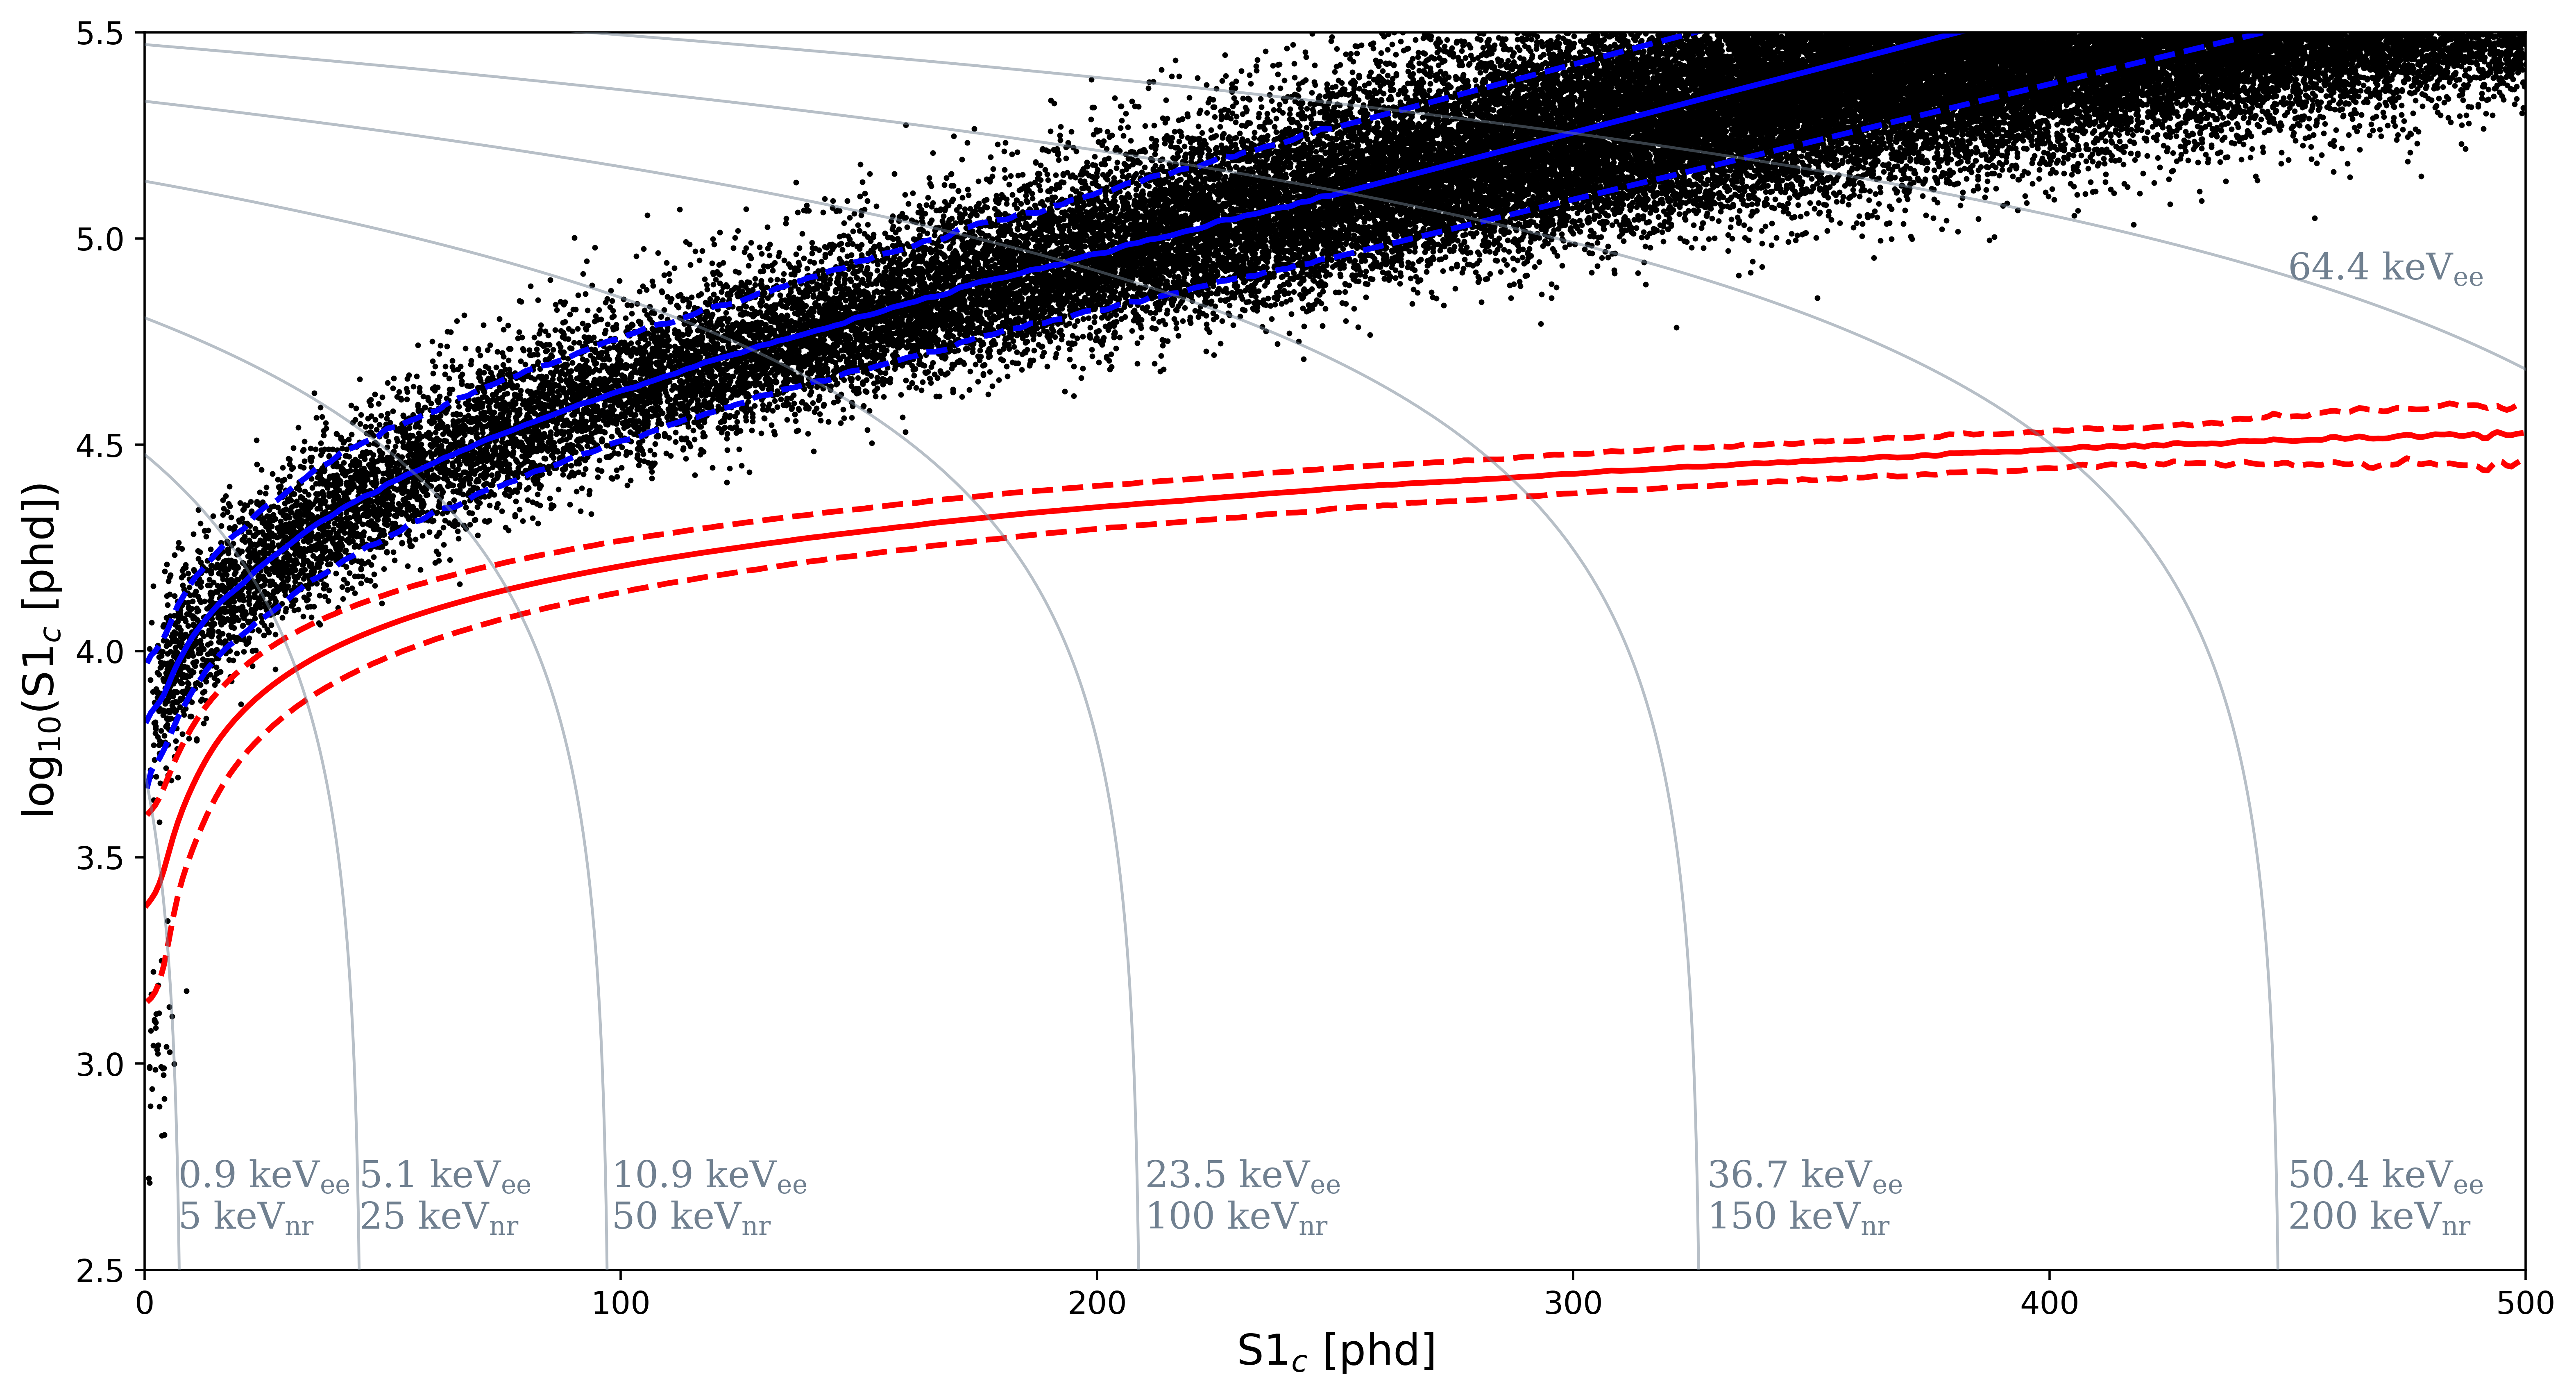
\includegraphics[width=15cm]{Figures/EFT/Projected_backgrounds/projected_backgrounds_s1_s2.png}
    \caption{Simulated data set for a background-only 1000 live day run with a 5.6-tonne fiducial mass. The ER and NR bands are shown in blue and red, respectively; the solid lines are the mean, and the dashed are 10\% and 90\% quantiles.}
    \label{fig:projected_background_dataset}
\end{figure}

\subsection{Projected Sensitivity}
\par
Presented in \autoref{fig:EFT_Result_Projected_Sensitivity_1} and \autoref{fig:EFT_Result_Projected_Sensitivity_2} are the projected sensitivities from a one-sided PLR test statistic.
A one-sided PLR was chosen over using a two-sided test as the purpose is to determine the sensitivity of LZ to the couplings, $c^s_i$, not the discovery significance. 
This approach is also in line with that used for the SI and SD projected sensitivity studies \cite{LZ_projected_sensitivity_paper_ref} as well a other sensitivity studies within LZ \cite{LZ_Ibles_LZStats_Thesis_ref, umituktu_thesis_ref}.
The -2$\sigma$ is excluded from the plot as the limit will be power contained \cite{power_constrained_limits_ref}, again a reporting style adopted from \cite{LZ_projected_sensitivity_paper_ref}.
Included in the figures are the XENON100 \cite{xenon100_eft_ref} and LUX \cite{LUX_RUN4_EFT_2021} limits.
Only a single data point is shown from LUX as their analysis was originally done in an \{$neutron,proton$\} basis for elastic operators and only reported an $isoscalar$ limit for a single WIMP mass for each operator.
\par
The sensitivity projections are presented in terms of the dimensionless values $({c}^{s}_{i}\times{m}^{2}_{w})^{2}$ where $m_w$ is the Higg's vacuum expectation value.
${c}^{s}_{i}$ has a dimensionality of [mass]$^{-2}$, which originates from the decision of the authors of \textit{DMFormFactor} to normalise spinors to unity, to use dimensionless representations of the operators and to scale the couplings by $m^{-2}_w$.
Reporting results in this format mirrors the LUX and XENON100 approach, allowing for a direct comparison.
\par
The parameter space to which the LZ detector is sensitive represents a significant step forward compared to current limits, improving by typically 3-4 orders of magnitude.
This is largely driven by the increased exposure of LZ with 5.6 tonnes $\times$ 1000 live days, compared to 34 kg $\times$ 224.6 live days from XENON100 and 100 kg $\times$ 311.2 live days from LUX.
The level of $\gamma$-X events will be the primary hold back to any potential discovery in the EFT region, but assuming that they can be successfully modelled in a more complex PLR, LZ has a very high projected sensitivity to EFT signatures.

\begin{figure}[!htbp]%
\centering
\begin{tikzpicture}
\centering
  \begin{groupplot}[view={0}{90},
    group style = {group size = 2 by 4,
                   vertical sep=1.5cm,
                   horizontal sep=2.0cm}]
    
    \pgfplotsforeachungrouped \x in {1,3,4,5,6,7,8,9}{
     \edef\tmp{
        \noexpand \nextgroupplot[
                                xlabel=Mass (MeV),
                                ylabel=$({c}^{s}_{\x}\times{m}^{2}_{w})^{2}$,
                                mark size=0pt,
                                width=0.45\textwidth,
                                height=5.5cm,
                                xmode=log,
                                ymode=log,
                                yminorticks=true,
                                x label style={at={(axis description cs:0.75,-0.1)},anchor=near ticklabel},
                                y label style={at={(axis description cs:-0.13,.75)},anchor=near ticklabel},
                                ]
            
            \noexpand \addplot[blue, name path = xenon100] table[]
                      {Data/HENR/Xenon100/O\x.dat};
                        
            \noexpand \addplot[only marks, mark size=1, error bars/.cd,
                               y dir=both, y explicit, error bar style={color=black}]
                               table[x=mass,y=median, y error plus index=3, y error minus index=2] {Data/HENR/Projected_Sensitivity/LUX/O\x.dat};
            
            \noexpand \addplot[green, opacity = 0.4, name path = nsig1] table[x=mass, y=nsig1]
                      {Data/HENR/Projected_Sensitivity/Results_method1/O\x.dat};
                      
            \noexpand \addplot[green, opacity = 0.4, name path = psig1] table[x=mass, y=psig1]
                      {Data/HENR/Projected_Sensitivity/Results_method1/O\x.dat};
                      
            \noexpand \addplot[yellow, opacity = 0.4, name path = psig2] table[x=mass, y=psig2]
                      {Data/HENR/Projected_Sensitivity/Results_method1/O\x.dat};
                      
            \noexpand \addplot[green, opacity = 0.4, forget plot] fill between[of=nsig1 and psig1];
            \noexpand \addplot[yellow, opacity = 0.4, forget plot] fill between[of=psig1 and psig2];
            
            \noexpand \addplot[black, name path = median] table[x=mass, y=median]
                      {Data/HENR/Projected_Sensitivity/Results_method1/O\x.dat};
            
            %\noexpand \addplot[black, dashed, name path = median] table[x=mass, y=cl]
            %          {Data/HENR/Projected_Sensitivity/Results/O\x.dat};
                     
        }
        \tmp 
        }
  \end{groupplot}
\end{tikzpicture}
\caption{}
\label{fig:EFT_Result_Projected_Sensitivity_1}
\end{figure}



\begin{figure}[!htbp]%
\centering
\begin{tikzpicture}
\centering
  \begin{groupplot}[view={0}{90},
    group style = {group size = 2 by 3,
                   vertical sep=1.5cm,
                   horizontal sep=2.0cm}]
    
    \pgfplotsforeachungrouped \x in {10,11,12,13,14,15}{
     \edef\tmp{
        \noexpand \nextgroupplot[
                                xlabel=Mass (MeV),
                                ylabel=$({c}^{s}_{\x}\times{m}^{2}_{w})^{2}$,
                                mark size=0pt,
                                width=0.45\textwidth,
                                height=5.5cm,
                                xmode=log,
                                ymode=log,
                                x label style={at={(axis description cs:0.75,-0.1)},anchor=near ticklabel},
                                y label style={at={(axis description cs:-0.13,.75)},anchor=near ticklabel},
                                ]
            
            \noexpand \addplot[blue, name path = xenon100] table[]
                      {Data/HENR/Xenon100/O\x.dat};
            
            \noexpand \addplot[only marks, mark size=1, error bars/.cd,
                               y dir=both, y explicit, error bar style={color=black}]
                               table[x=mass,y=median, y error plus index=3, y error minus index=2] {Data/HENR/Projected_Sensitivity/LUX/O\x.dat};
                        
            \noexpand \addplot[green, opacity = 0.4, name path = nsig1] table[x=mass, y=nsig1]
                      {Data/HENR/Projected_Sensitivity/Results_method1/O\x.dat};
                      
            \noexpand \addplot[green, opacity = 0.4, name path = psig1] table[x=mass, y=psig1]
                      {Data/HENR/Projected_Sensitivity/Results_method1/O\x.dat};
                      
            \noexpand \addplot[yellow, opacity = 0.4, name path = psig2] table[x=mass, y=psig2]
                      {Data/HENR/Projected_Sensitivity/Results_method1/O\x.dat};
                      
            \noexpand \addplot[green, opacity = 0.4, forget plot] fill between[of=nsig1 and psig1];
            \noexpand \addplot[yellow, opacity = 0.4, forget plot] fill between[of=psig1 and psig2];
            
            \noexpand \addplot[black, name path = median] table[x=mass, y=median]
                      {Data/HENR/Projected_Sensitivity/Results_method1/O\x.dat};
            
            %\noexpand \addplot[black, dashed, name path = median] table[x=mass, y=cl]
            %          {Data/HENR/Projected_Sensitivity/Results/O\x.dat};
                     
        }
        \tmp 
        }
  \end{groupplot}
\end{tikzpicture}
\caption{}
\label{fig:EFT_Result_Projected_Sensitivity}
\end{figure}


\iffalse
\subsection{Signal Model}
\par
As mentioned in \autoref{chap:detection_theory}, the parameters for the Standard Halo Model (SHM) used for generated signal models within direct dark matter experiments has been standardised since mid-2021 \cite{standard_halo_model_conventions_ref}.
However, this study began before that date and so used the parameters previously used within the LZ collaboration, in \cite{LZ_projected_sensitivity_paper_ref,LZ_TechnicalDesignReview_ref,LZ_Ibles_LZStats_Thesis_ref}.
The parameters used are shown in \autoref{tab:projected_DMFormFactor_parameters}.
One interesting benefit of this, however, is that the parameters are exactly the same as those used by both Xenon100 \cite{xenon100_eft_ref} LUX RUN-4 EFT analysis \cite{LUX_RUN4_EFT_2021}.

\begin{table}[]
    \centering
    \begin{tabular}{c|c}
        Parameter         & Value  \\ \hline
        $\nu_0$           & 220$km s^{-1}$ \\
        $\nu_{esc}$       & 544$km s^{-1}$ \\
        $\rho_{\chi}$     & 0.3 $GeV/cm^{3}$ \\
        $|\nu_E|$         & 245 $km s^{-1}$ 
    \end{tabular}
    \caption{Standard Halo Model parameters used for projected sensitivity study.}
    \label{tab:projected_DMFormFactor_parameters}
\end{table}

\par
With the projected detector parameters, the observable quantities \{$S1_c,log(S2_c)$\}, for a selection of operators at a mass of 100 GeV / c$^2$ are shown in \autoref{fig:projected_detector_model_signal_pdfs}.

\begin{figure}[!htbp]%
\centering
    \begin{tikzpicture}
    \centering
        \begin{groupplot}[view={0}{90},
            group style = {group size = 1 by 3,
            horizontal sep=0.6cm}]
        \iffalse
        \nextgroupplot[
        width=15cm, height=8cm,
        xlabel=,
        ylabel={log$_10$(S2$_{c}$ [phd])},
        mark size=0pt,
        xmin=0, xmax=500,
        ymin=2.5, ymax=5.5,
        colormap={blackwhite}{color=(white) color=(black)}]
        
        \addplot3[
              surf,
              shader=flat corner,
        	  mesh/cols=40,
        	  mesh/ordering=rowwise,
            ] file {Data/HENR/Projected_Sensitivity/Signal/pdf/o1_m100_pdf.dat};
            
        \addplot[blue, ]
            table [x=bin, y=mean]
            {Data/HENR/Projected_Sensitivity/Signal/pdf/er_band.dat};     
        \addplot[blue, dashed]
            table [x=bin, y=high]
            {Data/HENR/Projected_Sensitivity/Signal/pdf/er_band.dat};     
        \addplot[blue, dashed]
            table [x=bin, y=low]
            {Data/HENR/Projected_Sensitivity/Signal/pdf/er_band.dat};     

        \addplot[red, ]
            table [x=bin, y=mean]
            {Data/HENR/Projected_Sensitivity/Signal/pdf/nr_band.dat};    
        \addplot[red, dashed]
            table [x=bin, y=high]
            {Data/HENR/Projected_Sensitivity/Signal/pdf/nr_band.dat};     
        \addplot[red, dashed]
            table [x=bin, y=low]
            {Data/HENR/Projected_Sensitivity/Signal/pdf/nr_band.dat};  
        
        \node[draw, fill=white] at (axis cs: 450,3) {\large $\Operator$1};    
        
        \fi
        \nextgroupplot[
        width=15cm, height=8cm,
        xlabel=,
        ylabel={log$_10$(S2$_{c}$ [phd])},
        mark size=0pt,
        xmin=0, xmax=500,
        ymin=2.5, ymax=5.5,
        colormap={blackwhite}{color=(white) color=(black)}]
        
        \addplot3[
              surf,
              shader=flat corner,
        	  mesh/cols=40,
        	  mesh/ordering=rowwise,
            ] file {Data/HENR/Projected_Sensitivity/Signal/pdf/o6_m100_pdf.dat};
            
        \addplot[blue, ]
            table [x=bin, y=mean]
            {Data/HENR/Projected_Sensitivity/Signal/pdf/er_band.dat};     
        \addplot[blue, dashed]
            table [x=bin, y=high]
            {Data/HENR/Projected_Sensitivity/Signal/pdf/er_band.dat};     
        \addplot[blue, dashed]
            table [x=bin, y=low]
            {Data/HENR/Projected_Sensitivity/Signal/pdf/er_band.dat};     

        \addplot[red, ]
            table [x=bin, y=mean]
            {Data/HENR/Projected_Sensitivity/Signal/pdf/nr_band.dat};    
        \addplot[red, dashed]
            table [x=bin, y=high]
            {Data/HENR/Projected_Sensitivity/Signal/pdf/nr_band.dat};     
        \addplot[red, dashed]
            table [x=bin, y=low]
            {Data/HENR/Projected_Sensitivity/Signal/pdf/nr_band.dat};  
            
        \node[draw, fill=white] at (axis cs: 450,3) {\large $\Operator$6};
        
        \nextgroupplot[
        width=15cm, height=8cm,
        xlabel={S1$_{c}$ [phd]},
        ylabel={log$_10$(S2$_{c}$ [phd])},
        mark size=0pt,
        xmin=0, xmax=500,
        ymin=2.5, ymax=5.5,
        colormap={blackwhite}{color=(white) color=(black)}]
        
        \addplot3[
              surf,
              shader=flat corner,
        	  mesh/cols=40,
        	  mesh/ordering=rowwise,
            ] file {Data/HENR/Projected_Sensitivity/Signal/pdf/o15_m100_pdf.dat};
            
        \addplot[blue, ]
            table [x=bin, y=mean]
            {Data/HENR/Projected_Sensitivity/Signal/pdf/er_band.dat};     
        \addplot[blue, dashed]
            table [x=bin, y=high]
            {Data/HENR/Projected_Sensitivity/Signal/pdf/er_band.dat};     
        \addplot[blue, dashed]
            table [x=bin, y=low]
            {Data/HENR/Projected_Sensitivity/Signal/pdf/er_band.dat};     

        \addplot[red, ]
            table [x=bin, y=mean]
            {Data/HENR/Projected_Sensitivity/Signal/pdf/nr_band.dat};    
        \addplot[red, dashed]
            table [x=bin, y=high]
            {Data/HENR/Projected_Sensitivity/Signal/pdf/nr_band.dat};     
        \addplot[red, dashed]
            table [x=bin, y=low]
            {Data/HENR/Projected_Sensitivity/Signal/pdf/nr_band.dat}; 
            
        \node[draw, fill=white] at (axis cs: 450,3) {\large $\Operator$15};
        
        \end{groupplot}
    \end{tikzpicture}
    \caption{Distribution of signal models in \{S1$_c$,log$_{10}$(S2$_c$) showing the variation between operators.
             Each pdf is shown for a WIMP mass of 100 GeV.}
    \label{fig:projected_detector_model_signal_pdfs}
\end{figure}

\fi